%=======================================================================
%  Laporan Proyek Algoritma Genetika - Wisata Genetik
%  File utama Overleaf: main.tex  (compiler: pdfLaTeX)
%=======================================================================
\documentclass[11pt]{article}

% ---------- Ukuran kertas & margin ----------
\usepackage[a4paper, top=2.1cm, bottom=2.1cm, left=2.4cm, right=2.4cm, footskip=1.0cm]{geometry}

% ---------- Font & bahasa ----------
\usepackage[T1]{fontenc}
\usepackage[utf8]{inputenc}
\usepackage{mathptmx}
\usepackage{microtype}
\linespread{1.07}

% ---------- Paket pendukung ----------
\usepackage{graphicx}
\usepackage{amsmath}
\usepackage{amssymb}
\usepackage{booktabs}
\usepackage{multirow}
\usepackage{array}
\usepackage{float}
\usepackage[font=small,labelfont=bf,skip=4pt]{caption}
\usepackage{subcaption}
\usepackage{enumitem}
\usepackage{titlesec}
\usepackage[section]{placeins}
\usepackage{indentfirst}
\usepackage{xurl}
\usepackage{xcolor}
\usepackage[hidelinks]{hyperref}
\usepackage{tikz}
\usetikzlibrary{positioning, arrows.meta, fit, backgrounds, calc}
\usepackage{pgfplots}
\pgfplotsset{compat=1.18, /pgf/number format/use comma}

% ---------- Warna identitas (sama dengan aplikasi) ----------
\definecolor{ugmnavy}{HTML}{0C2A56}
\definecolor{ugmgold}{HTML}{F5C400}
\definecolor{abu}{HTML}{94A3B8}

% ---------- Rujukan Gambar/Tabel yang seluruh tulisannya bisa diklik ----------
\newcommand{\Gambarref}[1]{\hyperref[#1]{Gambar~\ref*{#1}}}
\newcommand{\Tabelref}[1]{\hyperref[#1]{Tabel~\ref*{#1}}}

% ---------- Istilah bahasa Indonesia ----------
\renewcommand{\figurename}{Gambar}
\renewcommand{\tablename}{Tabel}
\renewcommand{\refname}{Daftar Pustaka}
\renewcommand{\contentsname}{Daftar Isi}

% ---------- Format judul bagian ----------
\titleformat{\section}{\normalfont\large\bfseries}{\thesection}{0.6em}{}
\titleformat{\subsection}{\normalfont\normalsize\bfseries}{\thesubsection}{0.6em}{}
\titlespacing*{\section}{0pt}{2.0ex plus .3ex minus .2ex}{1.0ex plus .2ex}
\titlespacing*{\subsection}{0pt}{1.6ex plus .3ex minus .2ex}{0.7ex plus .2ex}
\setlist[enumerate]{itemsep=1pt, topsep=2pt, parsep=0pt, leftmargin=1.6em}
\setlist[itemize]{itemsep=1pt, topsep=2pt, parsep=0pt, leftmargin=1.6em}
\setlength{\parindent}{1.2em}
\setlength{\textfloatsep}{8pt plus 2pt minus 2pt}
\setlength{\intextsep}{8pt plus 2pt minus 2pt}
\renewcommand{\arraystretch}{1.12}

% ---------- Nama mata kuliah (ubah di sini bila perlu) ----------
\newcommand{\matakuliah}{ALGORITMA GENETIKA (PACS262501)}

\begin{document}

%=======================================================================
% HALAMAN JUDUL
%=======================================================================
\begin{titlepage}
\centering
\thispagestyle{empty}
\vspace*{\fill}
\large

\textbf{LAPORAN PROYEK}\\
\textbf{\matakuliah}

\vspace{1.1cm}
\begin{minipage}{0.86\textwidth}
\centering\bfseries
OPTIMASI REKOMENDASI RENCANA PERJALANAN WISATA MENGGUNAKAN ALGORITMA GENETIKA
\end{minipage}

\vspace{1.1cm}

\includegraphics[width=6cm]{gambar/logo-ugm.png}

\vspace{1.1cm}
\textbf{DISUSUN OLEH:}\\[4pt]
Azhar Maulana (24/533487/PA/22582)\\
Kukuh Agus Hermawan (24/533395/PA/22573)

\vspace{1.1cm}
\textbf{PROGRAM STUDI ILMU KOMPUTER}\\
\textbf{DEPARTEMEN ILMU KOMPUTER DAN ELEKTRONIKA}\\
\textbf{FAKULTAS MATEMATIKA DAN ILMU PENGETAHUAN ALAM}\\
\textbf{UNIVERSITAS GADJAH MADA}\\
\textbf{SLEMAN, DAERAH ISTIMEWA YOGYAKARTA}\\
\textbf{SEMESTER GANJIL 2026/2027}
\vspace*{\fill}
\end{titlepage}

\tableofcontents
\thispagestyle{empty}
\newpage
\setcounter{page}{1}
\pagestyle{plain}

\section{Pendahuluan}

\subsection{Latar Belakang}

Layanan digital kini menjadi bagian dari cara orang merencanakan perjalanan. Pada 2020, Asia Tenggara memiliki sekitar 400 juta pengguna internet aktif dan 94\% di antaranya berniat tetap memakai layanan digital setelah pandemi \cite{econ2020}. Nilai transaksi perjalanan daring di Indonesia mencapai US\$9 miliar pada 2024, tumbuh 24\% per tahun \cite{econ2024}, sementara perjalanan wisatawan nusantara Januari--Agustus 2024 mencapai 674,6 juta, tumbuh 19,2\% \cite{bps2024}. Rekomendasi yang tepat menghemat waktu wisatawan dalam mencari dan memutuskan.

Namun, rekomendasi wisata tidak cukup hanya menebak destinasi yang disukai. Sistem harus menemukan \emph{kombinasi} destinasi beserta \emph{urutan} kunjungannya yang pas dengan anggaran, waktu, dan jumlah orang. Dari 201 destinasi terdapat $2^{201} \approx 3{,}2 \times 10^{60}$ kemungkinan himpunan destinasi, belum termasuk urutannya. Pendekatan \textit{greedy} (pilih yang termurah atau terdekat dulu) mudah terjebak pada pilihan yang tampak baik secara lokal. Algoritma Genetika (GA) \cite{holland1975, goldberg1989} cocok untuk masalah seperti ini karena menjelajahi banyak solusi sekaligus lewat populasi, diarahkan oleh fungsi fitness, dan konvergen ke solusi yang sangat baik dalam waktu singkat.

\subsection{Tujuan}

\begin{enumerate}
  \item Memodelkan rekomendasi rencana perjalanan sebagai gabungan masalah pemilihan (mirip Knapsack) dan pengurutan rute (mirip TSP), dengan batas anggaran dan waktu.
  \item Membangun GA lengkap tanpa pustaka GA siap pakai: representasi kromosom, fungsi fitness, seleksi, crossover, mutasi, elitisme, dan kriteria berhenti.
  \item Membuktikan efektivitas GA terhadap metode pembanding (dua varian greedy dan pencarian acak) serta menganalisis sensitivitas parameternya.
  \item Menyajikan hasilnya dalam aplikasi web interaktif yang dapat memakai dataset pengguna sendiri.
\end{enumerate}

\subsection{Sumber Kode}

Seluruh kode ditulis dalam TypeScript dan tersedia di \url{https://github.com/kukuhagushermawan/GA-rekomendasi}. Mesin GA berada di folder \texttt{src/ga/} dan dipisah per tahap agar mudah ditelusuri (\Tabelref{tab:kode}).

\begin{table}[H]
\centering
\caption{Pemetaan berkas kode ke isi laporan.}
\label{tab:kode}
\small
\begin{tabular}{@{}l >{\raggedright\arraybackslash}p{8.4cm} l@{}}
\toprule
\textbf{Berkas} & \textbf{Isi} & \textbf{Subbab} \\
\midrule
\texttt{data.ts}       & membaca dan memvalidasi dataset, menyusun matriks per nama & \ref{sec:data} \\
\texttt{kromosom.ts}   & representasi kromosom dua bagian dan dekodenya & \ref{sec:kromosom} \\
\texttt{fitness.ts}    & biaya, durasi, validitas, fitness, jadwal harian & \ref{sec:model}, \ref{sec:fitness} \\
\texttt{operator.ts}   & seleksi, crossover, dan mutasi & \ref{sec:operator} \\
\texttt{ga.ts}         & populasi awal, loop GA, elitisme, kriteria berhenti, top-5 & \ref{sec:operator} \\
\texttt{pembanding.ts} & greedy, pencarian acak, eksperimen & \ref{sec:eksperimen} \\
\texttt{worker.ts}     & menjalankan GA di Web Worker untuk aplikasi web & \ref{sec:implementasi} \\
\texttt{tests/ga.test.ts} & 37 uji unit & \ref{sec:verifikasi} \\
\bottomrule
\end{tabular}
\end{table}

\section{Metodologi}

\subsection{Data}
\label{sec:data}

Dataset bawaan berasal dari repositori kode makalah acuan \cite{qomariyah2021, repo} dan dipakai apa adanya tanpa data sintetis. Isinya:
\begin{itemize}
  \item \texttt{jsonAttraction.txt}: 201 atraksi di Jabodetabek, masing-masing dengan harga tiket masuk (HTM, rupiah per orang), lama kunjungan (jam), 1--5 tag kategori, dan koordinat. Sebanyak 92 atraksi gratis, median HTM Rp2.000, dan rata-rata lama kunjungan 1,52 jam.
  \item \texttt{distanceMatrix.csv} dan \texttt{durationMatrix.csv}: jarak jalan (meter) dan waktu tempuh (detik) antaratraksi dari Google Distance Matrix, berukuran $202 \times 202$ karena memuat satu label tambahan ``Jakarta''. Urutan barisnya tidak sama dengan urutan atraksi, sehingga sel matriks dicari berdasarkan nama.
\end{itemize}

Audit data menemukan delapan atraksi bermasalah: tujuh memiliki jarak lebih dari 100 km ke hampir semua atraksi lain (salah geokode, misalnya National Monument ke Museum of East Timor tercatat 3.096 km), dan satu tidak memiliki rute sama sekali (semua sel bernilai $-1$). Kedelapannya tidak dijadikan kandidat, sehingga GA bekerja dengan \textbf{193 kandidat}. Sel bernilai $-1$ atau 0 di luar diagonal diganti 15 km dan 1.300 detik, mengikuti aturan kode asli \cite{repo}. Delapan tag yang tersedia diberi label Indonesia untuk antarmuka: alam (81 atraksi), ramah anak (68), museum (43), seni \& budaya (31), sejarah (24), taman hiburan (21), pantai (9), dan favorit lokal (8).

Pengguna juga dapat mengunggah dataset sendiri dengan format yang sama. Setiap berkas divalidasi dengan skema \texttt{zod} sebelum dipakai, sehingga sistem tidak terbatas pada Jakarta.

\subsection{Model Masalah}
\label{sec:model}

Masukan pengguna adalah anggaran $B$, jumlah hari, jam per hari, jumlah orang $p$, dan bobot minat $w_t \in [0, 1]$ untuk setiap tag. Batas jam total adalah $T = \text{hari} \times \text{jam per hari}$. Sebuah rencana adalah rute berurutan $R = (r_1, \dots, r_m)$ tanpa destinasi ganda. Biaya dan durasinya:
\begin{align}
C &= p \sum_{i=1}^{m} \text{HTM}_{r_i} \;+\; 5.000 \left\lceil \tfrac{p}{4} \right\rceil \sum_{k=1}^{m-1} d_{r_k r_{k+1}}, \label{eq:biaya}\\
D &= \sum_{i=1}^{m} v_{r_i} \;+\; \sum_{k=1}^{m-1} t_{r_k r_{k+1}}, \label{eq:durasi}
\end{align}
dengan $d$ jarak (km), $t$ waktu tempuh (jam), $v$ lama kunjungan, dan Rp5.000/km tarif taksi dari kode asli \cite{repo}, satu taksi untuk setiap empat orang. Rencana dinyatakan
\begin{equation}
\textbf{VALID} \iff C \le B \;\wedge\; D \le T.
\end{equation}
Masalah ini menggabungkan \textbf{pemilihan} destinasi (mirip Knapsack) dan \textbf{pengurutan} rute (mirip TSP), sehingga representasi kromosom harus menangkap keduanya.

\subsection{Representasi Kromosom}
\label{sec:kromosom}

Kromosom terdiri dari dua bagian berukuran $n$ (jumlah kandidat): \texttt{mask}, larik biner yang menandai destinasi terpilih, dan \texttt{order}, permutasi seluruh kandidat yang menyatakan urutan relatif. Rute diperoleh dengan membaca \texttt{order} dari kiri dan mengambil kandidat yang \texttt{mask}-nya 1 (\Gambarref{fig:kromosom}).

\begin{figure}[H]
\centering
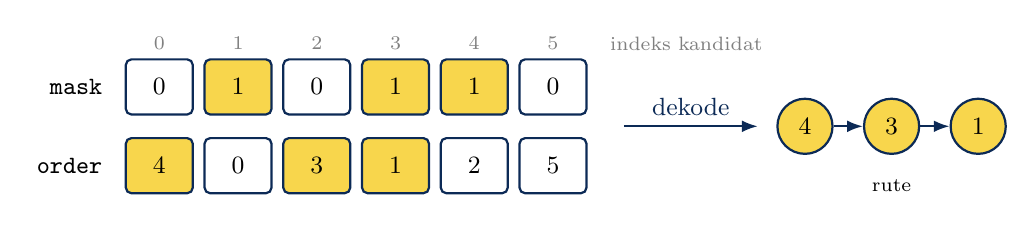
\begin{tikzpicture}[
  every node/.style={font=\small},
  gen/.style={rectangle, draw=ugmnavy, thick, minimum width=0.85cm, minimum height=0.7cm, rounded corners=2pt},
  pilih/.style={gen, fill=ugmgold!70},
  arr/.style={-{Latex[length=2mm]}, thick, ugmnavy}
]
\node[anchor=east] at (-0.2,1.0) {\texttt{mask}};
\node[anchor=east] at (-0.2,0) {\texttt{order}};
\foreach \i/\m in {0/0,1/1,2/0,3/1,4/1,5/0} {
  \ifnum\m=1 \node[pilih] (m\i) at (\i*1.0+0.4,1.0) {\m}; \else \node[gen] (m\i) at (\i*1.0+0.4,1.0) {\m}; \fi
  \node[font=\scriptsize, gray] at (\i*1.0+0.4,1.55) {\i};
}
\foreach \j/\g in {0/4,1/0,2/3,3/1,4/2,5/5} {
  \pgfmathtruncatemacro{\sel}{(\g==1 || \g==3 || \g==4) ? 1 : 0}
  \ifnum\sel=1 \node[pilih] (o\j) at (\j*1.0+0.4,0) {\g}; \else \node[gen] (o\j) at (\j*1.0+0.4,0) {\g}; \fi
}
\node[font=\scriptsize, gray, anchor=west] at (6.0,1.55) {indeks kandidat};
\draw[arr] (6.3,0.5) -- node[above]{dekode} (8.0,0.5);
\node[pilih, circle, minimum width=0.7cm] (r1) at (8.6,0.5) {4};
\node[pilih, circle, minimum width=0.7cm] (r2) at (9.7,0.5) {3};
\node[pilih, circle, minimum width=0.7cm] (r3) at (10.8,0.5) {1};
\draw[arr] (r1) -- (r2); \draw[arr] (r2) -- (r3);
\node[font=\scriptsize] at (9.7,-0.25) {rute};
\end{tikzpicture}
\caption{Kromosom dua bagian dengan $n = 6$. Kandidat 1, 3, dan 4 dipilih (kuning); urutannya dibaca dari \texttt{order}, sehingga rutenya $4 \to 3 \to 1$.}
\label{fig:kromosom}
\end{figure}

Representasi ini dipilih karena tiga alasan. Pertama, setiap kromosom selalu terdekode menjadi rute yang sah tanpa destinasi ganda, sehingga tidak perlu proses perbaikan. Kedua, operator standar dapat langsung dipakai pada bagian yang sesuai: crossover biner pada \texttt{mask} dan \textit{order crossover} pada \texttt{order}. Ketiga, posisi kandidat yang sedang tidak dipilih tetap diwariskan, sehingga ketika kandidat itu dipilih kembali, letaknya di rute sudah ``teringat''.

\subsection{Fungsi Fitness}
\label{sec:fitness}

Fitness mengikuti makalah acuan \cite{qomariyah2021}, yaitu kebalikan dari jumlah kesalahan biaya dan durasi terhadap targetnya. Kesalahan dihitung relatif agar biaya (rupiah) dan durasi (jam) setara:
\begin{equation}
\text{cost\_score} = \frac{|C - B|}{B}, \qquad \text{duration\_score} = \frac{|D - T|}{T}.
\end{equation}
Fungsi akhirnya menambahkan penalti pelanggaran batas dan bonus kecocokan minat:
\begin{equation}
\text{fitness} = \frac{1 + w_p \cdot \text{minat}}{\varepsilon + \text{cost\_score} + \text{duration\_score} + w_v\!\left(\frac{\max(0, C-B)}{B} + \frac{\max(0, D-T)}{T}\right) + w_s \frac{O}{T}},
\label{eq:fitness}
\end{equation}
dengan $O$ kelebihan jam jadwal harian (Subbab~\ref{sec:jadwal}). Skor minat sebuah destinasi adalah bobot tertinggi di antara tag-nya dibagi bobot maksimum masukan, dan \textit{minat} rencana adalah rata-ratanya. Bobot bawaannya $w_v = 10$, $w_s = 1$, $w_p = 1$, dan $\varepsilon = 0{,}01$. Penalti $w_v = 10$ membuat pelanggaran sebelas kali lebih mahal daripada kekurangan dengan selisih yang sama, sehingga GA terdorong ke sisi valid. Kekurangan tetap dihukum karena tujuannya adalah titik \emph{paling seimbang}: rencana yang memanfaatkan anggaran dan waktu sebaik mungkin tanpa melanggarnya. Dengan $w_v = w_s = w_p = 0$, Persamaan~(\ref{eq:fitness}) kembali menjadi rumus makalah acuan.

\subsection{Operator Genetika}
\label{sec:operator}

\textbf{Populasi awal.} Dari 100 individu, 20\% dibangun dengan \textit{greedy seeding}: mulai dari kandidat acak (berbobot minat), lalu berulang kali memilih acak satu dari lima kandidat terdekat yang masih layak (biaya $\le B$, durasi $\le T$, dan jadwal harian tetap muat). Individu ini selalu valid, sehingga populasi awal tidak seluruhnya tidak valid. Sisanya berisi $k \sim U[1, k_{\max}]$ kandidat acak, dengan $k_{\max}$ perkiraan jumlah destinasi yang muat dalam $T$.

\textbf{Seleksi.} Tersedia seleksi turnamen dengan $k = 3$ (bawaan), yaitu tiga individu diambil acak lalu yang fitness-nya tertinggi menang, dan \textit{roulette wheel} dengan peluang $f_i / \sum_j f_j$.

\textbf{Crossover} (peluang 0,8). Bagian \texttt{mask} memakai \textit{uniform crossover} (tiap bit ditukar dengan peluang $\tfrac12$) atau \textit{one-point}. Bagian \texttt{order} memakai \textit{order crossover} (OX) \cite{davis1985}: segmen acak disalin dari induk pertama, lalu posisi lain diisi gen induk kedua sesuai urutannya (\Gambarref{fig:ox}). Anaknya selalu berupa permutasi yang sah.

\begin{figure}[H]
\centering
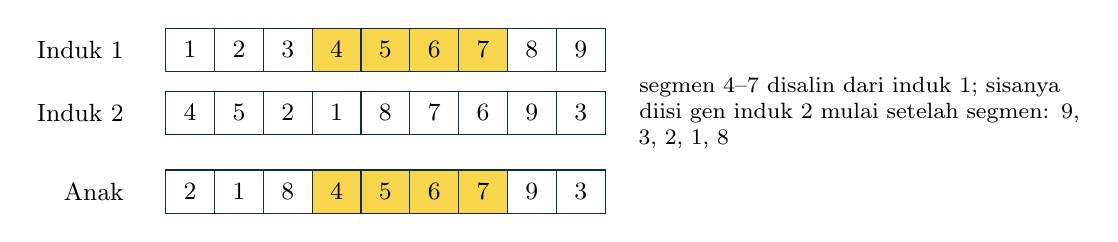
\begin{tikzpicture}[
  every node/.style={font=\small},
  sel/.style={rectangle, draw=ugmnavy, minimum width=0.62cm, minimum height=0.55cm},
  seg/.style={sel, fill=ugmgold!70},
]
\foreach \row/\label/\vals/\a/\b in {0/Induk 1/{1,2,3,4,5,6,7,8,9}/4/7, -0.8/Induk 2/{4,5,2,1,8,7,6,9,3}/0/0, -1.8/Anak/{2,1,8,4,5,6,7,9,3}/4/7} {
  \node[anchor=east] at (-0.1,\row) {\label};
  \foreach \v [count=\c] in \vals {
    \pgfmathtruncatemacro{\inseg}{(\c>=\a && \c<=\b) ? 1 : 0}
    \ifnum\inseg=1 \node[seg] at (\c*0.62,\row) {\v}; \else \node[sel] at (\c*0.62,\row) {\v}; \fi
  }
}
\node[anchor=west, font=\footnotesize, text width=5.6cm] at (6.2,-0.8) {segmen 4--7 disalin dari induk 1; sisanya diisi gen induk 2 mulai setelah segmen: 9, 3, 2, 1, 8};
\end{tikzpicture}
\caption{Contoh \textit{order crossover} \cite{davis1985}.}
\label{fig:ox}
\end{figure}

\textbf{Mutasi} (peluang 0,05 per destinasi di rute). Satu dari empat operator dipilih acak: \textit{swap} (tukar dua destinasi), \textit{insert} (pindahkan satu destinasi), \textit{tambah}, dan \textit{hapus}. Mutasi tambah memilih salah satu dari sepuluh tetangga terdekat sebuah destinasi di rute dengan peluang 0,8 dan menyisipkannya tepat setelah destinasi itu. Dengan cara ini mutasi tidak membuat rute memutar jauh.

\textbf{Elitisme dan kriteria berhenti.} Dua individu terbaik disalin utuh ke generasi berikutnya, sehingga fitness terbaik tidak pernah turun. GA berhenti setelah 200 generasi atau bila fitness terbaik tidak membaik selama 100 generasi.

\textbf{Keluaran.} Selama run, rencana terbaik disimpan per himpunan destinasi. Lima rencana diambil dengan urutan: valid lebih dulu, lalu yang jadwal hariannya muat, lalu fitness tertinggi, dengan syarat setiap pasangan berbeda minimal dua destinasi. \Tabelref{tab:parameter} merangkum parameter bawaan, dan semuanya dapat diubah dari antarmuka.

\begin{table}[H]
\centering
\caption{Parameter bawaan GA.}
\label{tab:parameter}
\small
\begin{tabular}{@{}l l l@{}}
\toprule
\textbf{Parameter} & \textbf{Nilai} & \textbf{Keterangan} \\
\midrule
Ukuran populasi & 100 & 20\% greedy seeding, 80\% acak \\
Generasi maksimum & 200 & berhenti lebih awal bila stagnan 100 generasi \\
Seleksi & turnamen, $k = 3$ & alternatif: roulette wheel \\
Peluang crossover & 0,8 & uniform (\texttt{mask}) + OX (\texttt{order}) \\
Peluang mutasi & 0,05 & per destinasi di rute \\
Elitisme & 2 & individu terbaik disalin utuh \\
Seed acak & 42 & generator mulberry32, hasil dapat direproduksi \\
\bottomrule
\end{tabular}
\end{table}

\subsection{Jadwal Harian}
\label{sec:jadwal}

Rute dipecah ke hari-hari secara berurutan. Sebuah destinasi masuk ke hari berjalan bila jam hari itu ditambah waktu tempuh dan lama kunjungannya tidak melebihi jam per hari. Jika melebihi, hari baru dimulai. Waktu tempuh dari destinasi terakhir hari sebelumnya dihitung di awal hari berikutnya, sehingga total jam semua hari sama dengan $D$. Jadwal dinyatakan muat bila jumlah harinya tidak melebihi jumlah hari yang tersedia dan tidak ada hari yang melewati batas. Kelebihannya menjadi $O$ pada Persamaan~(\ref{eq:fitness}).

\subsection{Metode Pembanding dan Desain Eksperimen}
\label{sec:eksperimen}

GA dibandingkan dengan tiga metode yang memakai fungsi fitness yang sama:
\begin{itemize}
  \item \textbf{Greedy termurah dulu}: mulai dari destinasi dengan HTM termurah, lalu berulang kali menambah destinasi layak dengan biaya tambahan terkecil.
  \item \textbf{Greedy terdekat dulu}: mulai dari destinasi acak, lalu berulang kali menambah destinasi layak yang terdekat.
  \item \textbf{Pencarian acak}: membangkitkan rute acak sebanyak jumlah evaluasi GA pada seed yang sama (paling banyak 19.700), lalu mengambil yang terbaik.
\end{itemize}
Setiap metode dijalankan dengan seed 1--20 pada tiga skenario (\Tabelref{tab:skenario}). Analisis sensitivitas mengubah satu parameter dan menjaga parameter lain tetap bawaan, masing-masing dengan 10 seed pada skenario 1.

\begin{table}[H]
\centering
\caption{Skenario eksperimen.}
\label{tab:skenario}
\small
\begin{tabular}{@{}c l l l@{}}
\toprule
\textbf{No.} & \textbf{Anggaran dan waktu} & \textbf{Orang} & \textbf{Minat} \\
\midrule
1 & Rp1.000.000; 5 hari $\times$ 7 jam & 2 & -- \\
2 & Rp3.000.000; 3 hari $\times$ 10 jam & 2 & museum, pantai, ramah anak \\
3 & Rp500.000; 2 hari $\times$ 7 jam & 4 & alam \\
\bottomrule
\end{tabular}
\end{table}

\subsection{Implementasi}
\label{sec:implementasi}

Mesin GA ditulis sendiri dalam TypeScript tanpa pustaka GA. Aplikasi web dibangun dengan Next.js, React, Tailwind CSS, shadcn/ui, Apache ECharts untuk grafik, dan Leaflet dengan peta OpenStreetMap. GA dijalankan di Web Worker agar antarmuka tidak membeku dan progres per generasi dapat ditampilkan langsung. Parameter formulir disimpan di URL sehingga hasil dapat dibagikan dan direproduksi, karena seed yang sama selalu menghasilkan rencana yang sama.

\section{Hasil}

\subsection{Verifikasi Implementasi}
\label{sec:verifikasi}

Seluruh 37 uji unit lolos (\Tabelref{tab:uji}). Uji fitness dan validasi memakai angka dari data asli. Contohnya, rute National Monument $\to$ Merdeka Square $\to$ Irian Jaya Liberation Monument untuk dua orang berbiaya Rp58.095 dengan durasi 1,45 jam. Rute ini dinyatakan VALID untuk anggaran Rp60.000 dan batas 2 jam, tetapi TIDAK VALID bila anggarannya Rp58.000 atau batas jamnya 1,4 jam.

\begin{table}[H]
\centering
\caption{Uji unit pada \texttt{tests/ga.test.ts}.}
\label{tab:uji}
\small
\begin{tabular}{@{}l c >{\raggedright\arraybackslash}p{9.6cm}@{}}
\toprule
\textbf{Kelompok} & \textbf{Uji} & \textbf{Yang diuji} \\
\midrule
Data & 4 & 201 atraksi, matriks dicari per nama, format CSV, penolakan data tidak sah \\
Fitness dan validasi & 10 & biaya, durasi, VALID/TIDAK VALID, rumus fitness, penalti, bonus minat, jadwal harian \\
Kromosom & 3 & dekode, penulisan ulang urutan, penyandian rute \\
Crossover & 3 & OX mereproduksi contoh Davis \cite{davis1985}, anak selalu permutasi sah, uniform/one-point \\
Mutasi & 4 & swap, insert, tambah (termasuk tambah-lokal), hapus, kromosom tetap sah \\
Seleksi & 2 & frekuensi menang turnamen dan roulette sesuai teori \\
Loop GA & 8 & greedy seeding selalu valid, elitisme tidak pernah menurunkan fitness terbaik, determinisme seed, top-5 berbeda, stagnasi \\
Pembanding & 3 & greedy menghasilkan rute valid, pencarian acak memakai jumlah evaluasi yang sama \\
\midrule
\textbf{Total} & \textbf{37} & semua lolos \\
\bottomrule
\end{tabular}
\end{table}

Uji elitisme disertai uji pembanding: tanpa elitisme (seleksi roulette, elit 0), fitness terbaik terbukti bisa turun antargenerasi. Dengan begitu, lolosnya uji elitisme memang bermakna.

\subsection{Contoh Rekomendasi}

\Gambarref{fig:hasil} memperlihatkan hasil untuk skenario 1 dengan minat museum (bobot 1) dan sejarah (bobot 0,5), seed 42. GA selesai 200 generasi (19.700 evaluasi) dalam 0,36 detik. Kelima rencana VALID, hampir menghabiskan anggaran, dan jadwalnya muat dalam 5 hari (\Tabelref{tab:top5}).

\begin{figure}[H]
\centering
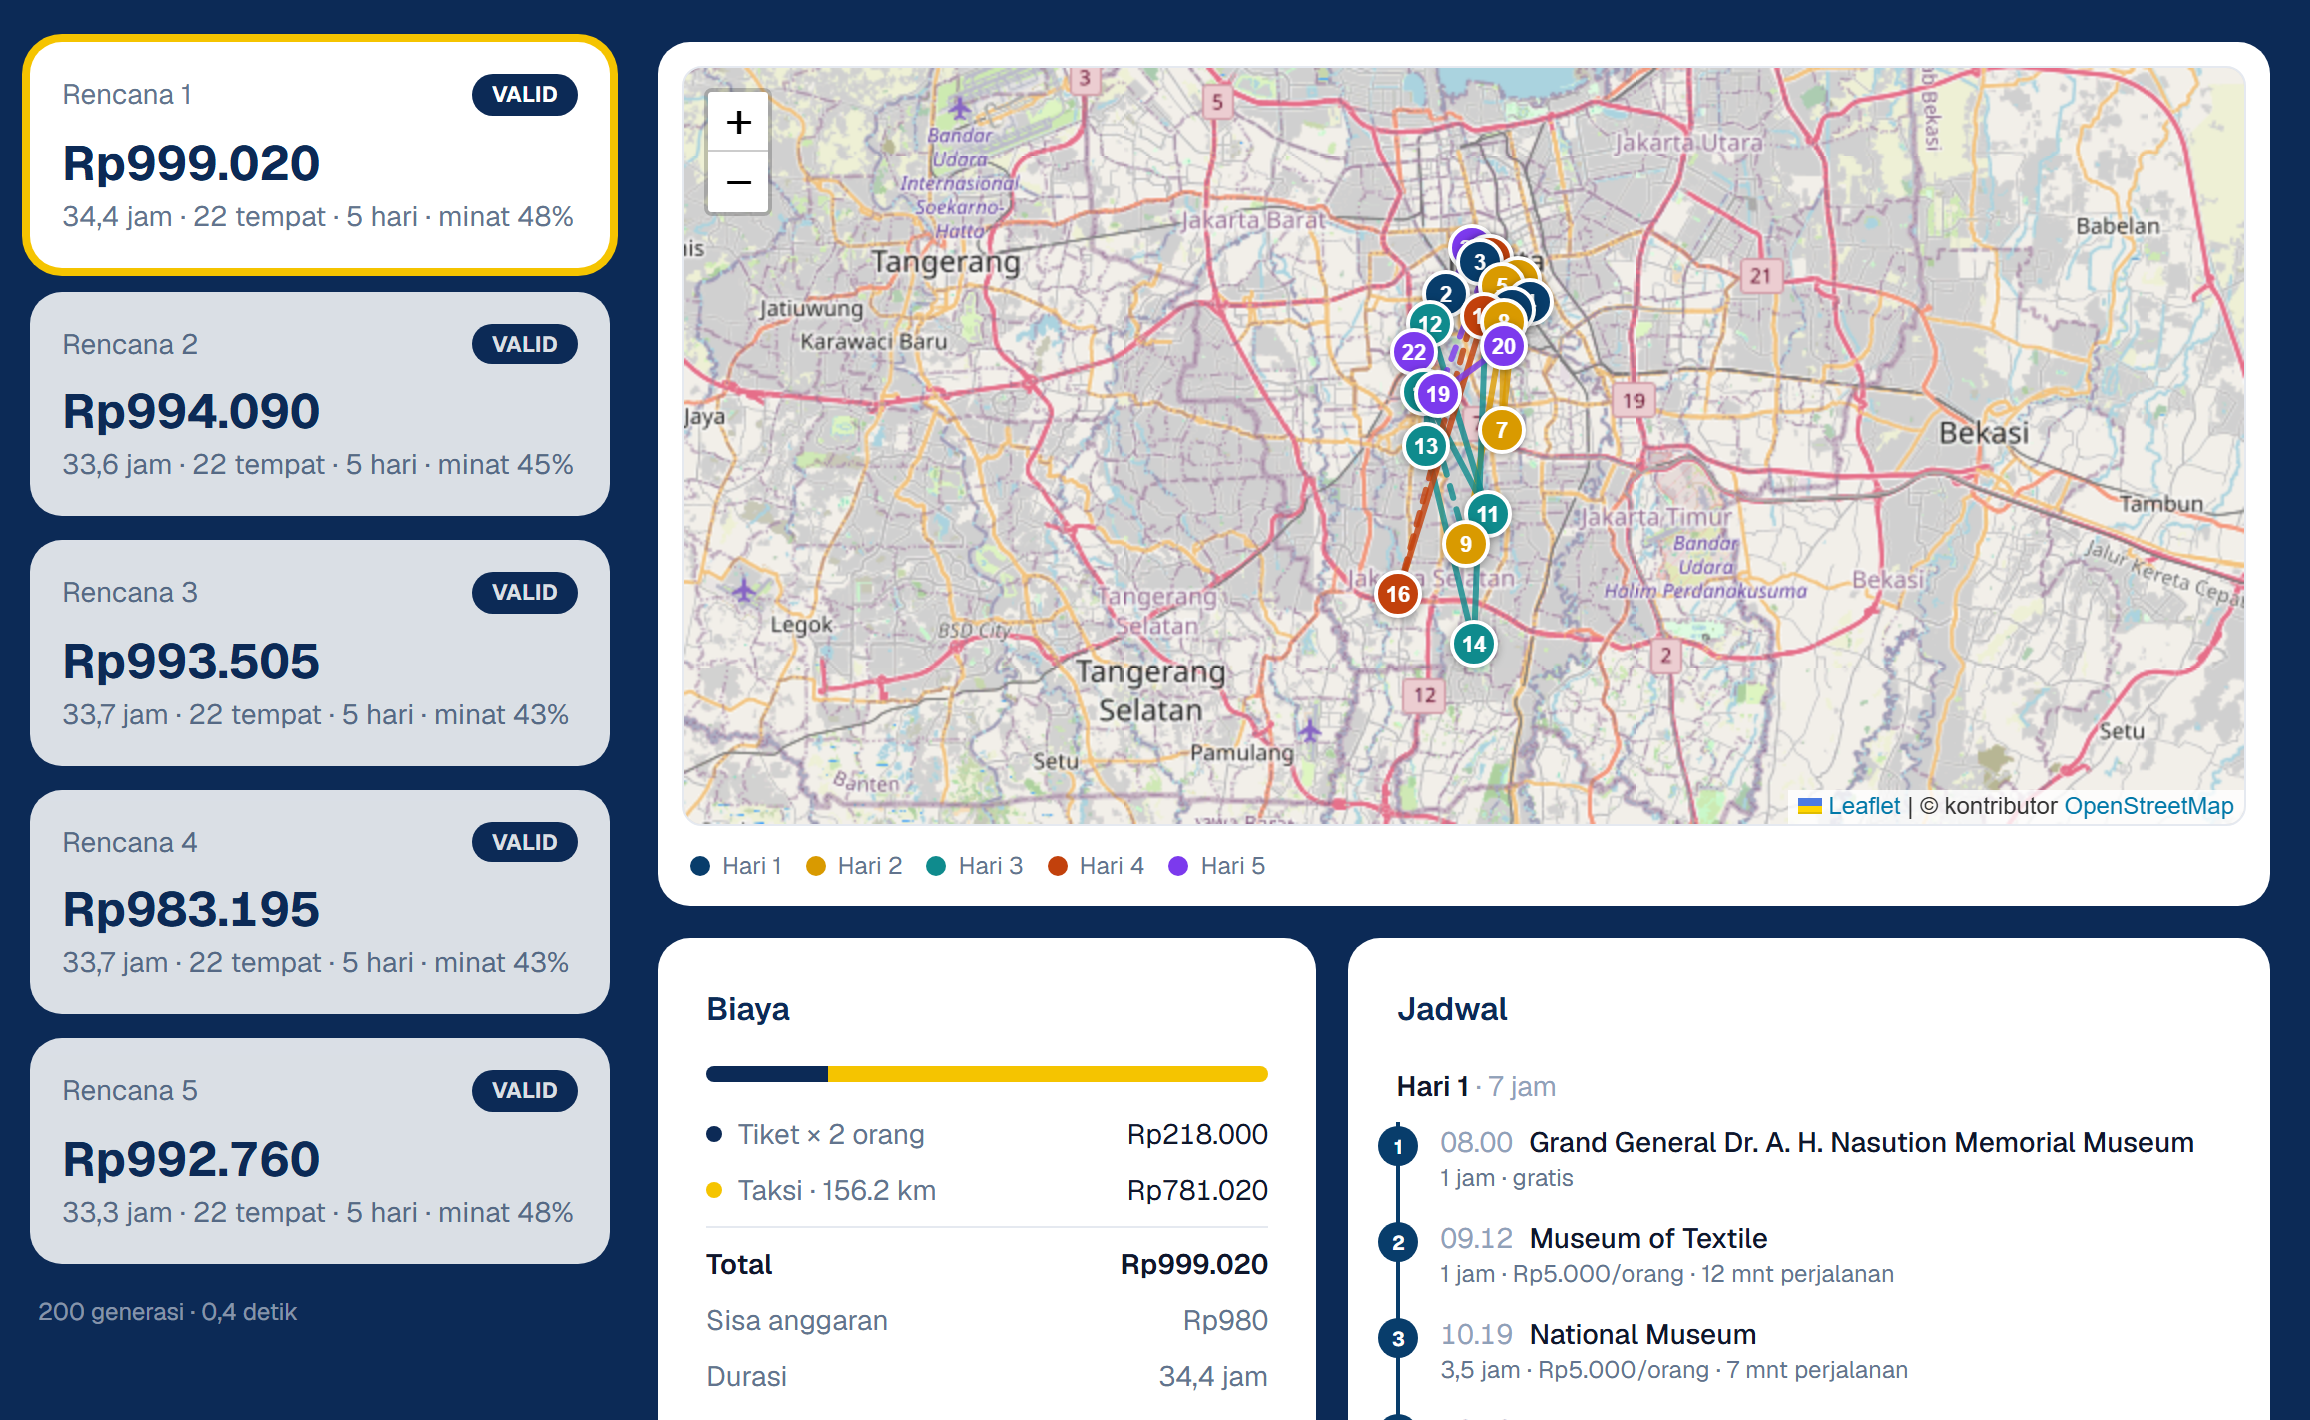
\includegraphics[width=\linewidth]{gambar/hasil-ringkas.png}
\caption{Halaman hasil aplikasi: lima rencana terbaik, peta rute berurutan (warna = hari), rincian biaya, dan jadwal harian.}
\label{fig:hasil}
\end{figure}

\begin{table}[H]
\centering
\caption{Lima rencana terbaik (Rp1.000.000; 5 hari $\times$ 7 jam; 2 orang; minat museum dan sejarah).}
\label{tab:top5}
\small
\begin{tabular}{@{}c r r c c c c c@{}}
\toprule
\textbf{Rencana} & \textbf{Biaya} & \textbf{Sisa} & \textbf{Durasi} & \textbf{Tempat} & \textbf{Minat} & \textbf{Fitness} & \textbf{Status} \\
\midrule
1 & Rp999.020 & Rp980    & 34,4 jam & 22 & 48\% & \textbf{50,73} & VALID \\
2 & Rp994.090 & Rp5.910  & 33,6 jam & 22 & 45\% & 26,49 & VALID \\
3 & Rp993.505 & Rp6.495  & 33,7 jam & 22 & 43\% & 26,01 & VALID \\
4 & Rp983.195 & Rp16.805 & 33,7 jam & 22 & 43\% & 22,54 & VALID \\
5 & Rp992.760 & Rp7.240  & 33,3 jam & 22 & 48\% & 22,46 & VALID \\
\bottomrule
\end{tabular}
\end{table}

Rencana 1 terdiri dari 29,25 jam kunjungan dan 5,12 jam perjalanan (156,2 km). Biayanya Rp218.000 untuk tiket dua orang dan Rp781.020 untuk taksi. Jadwalnya terbagi menjadi 4, 5, 6, 3, dan 4 destinasi per hari, masing-masing 6,7--7,0 jam. Hari pertama berisi empat destinasi bertema museum yang saling berdekatan: Grand General Dr.\ A.\ H.\ Nasution Memorial Museum, Museum of Textile (12 menit perjalanan), National Museum (7 menit), dan Jakarta Planetarium (9 menit).

\subsection{Konvergensi}

Fitness terbaik naik dari 11,77 pada generasi awal menjadi 50,73 pada generasi 200 (\Gambarref{fig:konvergensi}), atau 4,3 kali. Kurva terbaik tidak pernah turun karena elitisme dan naik bertahap setiap kali GA menemukan kombinasi yang lebih seimbang. Rata-rata fitness populasi naik dari 1,42 menjadi 6,10, sedangkan porsi individu valid naik dari 44\% menjadi 58\%.

\begin{figure}[H]
\centering
\begin{tikzpicture}
\begin{axis}[
  width=0.9\linewidth, height=6.2cm, xmin=0, xmax=200, ymin=0, ymax=60,
  xlabel={Generasi}, ylabel={Fitness}, axis y line*=left,
  legend style={at={(0.02,0.98)}, anchor=north west, font=\footnotesize, draw=none, fill=white, fill opacity=0.85, text opacity=1},
  tick label style={font=\footnotesize}, label style={font=\small}, grid=major, grid style={gray!15}]
\addplot[ugmnavy, very thick, const plot] table[x=gen, y=terbaik]{data/konvergensi.dat};
\addlegendentry{Fitness terbaik}
\addplot[ugmgold!85!black, thick] table[x=gen, y=ratarata]{data/konvergensi.dat};
\addlegendentry{Fitness rata-rata}
\addlegendimage{abu, dashed}
\addlegendentry{Individu valid (\%)}
\end{axis}
\begin{axis}[
  width=0.9\linewidth, height=6.2cm, xmin=0, xmax=200, ymin=0, ymax=100,
  axis y line*=right, axis x line=none, ylabel={Individu valid (\%)},
  tick label style={font=\footnotesize}, label style={font=\small}]
\addplot[abu, dashed] table[x=gen, y=valid]{data/konvergensi.dat};
\end{axis}
\end{tikzpicture}
\caption{Fitness terbaik dan rata-rata per generasi serta porsi individu valid (skenario pada \Tabelref{tab:top5}).}
\label{fig:konvergensi}
\end{figure}

\Gambarref{fig:sebaran} menunjukkan error biaya dan error durasi tiap individu pada populasi akhir. Keduanya saling tarik-menarik: rencana yang tepat waktu bisa boros biaya, dan sebaliknya. Individu yang paling seimbang hanya meleset 0,64 jam dan Rp980 dari target.

\begin{figure}[H]
\centering
\begin{tikzpicture}
\begin{axis}[
  width=0.9\linewidth, height=6cm, xmin=0, xmax=7, ymin=0, ymax=220,
  xlabel={$|$error durasi$|$ (jam)}, ylabel={$|$error biaya$|$ (Rp ribu)},
  legend style={at={(0.98,0.98)}, anchor=north east, font=\footnotesize, draw=none, fill=white, fill opacity=0.85, text opacity=1},
  tick label style={font=\footnotesize}, label style={font=\small}, grid=major, grid style={gray!15}]
\addplot[only marks, mark=*, mark size=1.7pt, ugmnavy] table[x=jam, y=biaya]{data/sebaran-valid.dat};
\addlegendentry{Valid}
\addplot[only marks, mark=*, mark size=1.4pt, abu!70] table[x=jam, y=biaya]{data/sebaran-tidak.dat};
\addlegendentry{Tidak valid}
\addplot[only marks, mark=*, mark size=4pt, ugmgold, draw=ugmnavy] table[x=jam, y=biaya]{data/sebaran-seimbang.dat}
  node[pos=0, anchor=west, font=\footnotesize\bfseries, ugmnavy, xshift=6pt, yshift=12pt, fill=white, inner sep=1pt] {paling seimbang};
\addlegendentry{Paling seimbang}
\end{axis}
\end{tikzpicture}
\caption{Error biaya terhadap error durasi pada populasi akhir. Sumbu dipotong pada persentil 90 agar klaster utama terlihat.}
\label{fig:sebaran}
\end{figure}

\subsection{Perbandingan dengan Metode Lain}

\Tabelref{tab:banding} dan \Gambarref{fig:banding} merangkum 20 run untuk setiap metode dan skenario. Semua metode selalu menghasilkan rencana valid, tetapi kualitasnya sangat berbeda. Fitness rata-rata GA \textbf{5,9; 3,8; dan 4,5 kali} pembanding terbaik pada skenario 1, 2, dan 3.

\begin{table}[H]
\centering
\caption{Perbandingan metode (rata-rata 20 seed). Pencarian acak memakai jumlah evaluasi yang sama dengan GA.}
\label{tab:banding}
\small
\setlength{\tabcolsep}{4.5pt}
\begin{tabular}{@{}c l r r r r r@{}}
\toprule
\textbf{Sk.} & \textbf{Metode} & \textbf{Fitness} & \textbf{Terbaik} & \textbf{Biaya} & \textbf{Durasi} & \textbf{Waktu} \\
\midrule
\multirow{4}{*}{1} & \textbf{Algoritma Genetika} & \textbf{22,62} $\pm$ 4,88 & \textbf{31,13} & Rp996.297 & 33,9 jam & 609 ms \\
 & Greedy termurah dulu & 1,09 $\pm$ 0,00 & 1,09 & Rp216.345 & 30,6 jam & $<$1 ms \\
 & Greedy terdekat dulu & 3,77 $\pm$ 2,18 & 9,46 & Rp847.777 & 28,7 jam & $<$1 ms \\
 & Pencarian acak & 3,82 $\pm$ 0,55 & 4,93 & Rp972.738 & 27,4 jam & 997 ms \\
\midrule
\multirow{4}{*}{2} & \textbf{Algoritma Genetika} & \textbf{82,62} $\pm$ 20,84 & \textbf{126,99} & Rp2.994.914 & 29,7 jam & 590 ms \\
 & Greedy termurah dulu & 1,50 $\pm$ 0,00 & 1,50 & Rp203.970 & 29,0 jam & $<$1 ms \\
 & Greedy terdekat dulu & 2,62 $\pm$ 1,57 & 6,88 & Rp1.173.908 & 26,9 jam & $<$1 ms \\
 & Pencarian acak & 21,64 $\pm$ 7,78 & 41,44 & Rp2.941.828 & 28,8 jam & 1.038 ms \\
\midrule
\multirow{4}{*}{3} & \textbf{Algoritma Genetika} & \textbf{76,25} $\pm$ 25,58 & \textbf{122,68} & Rp498.033 & 13,8 jam & 396 ms \\
 & Greedy termurah dulu & 1,80 $\pm$ 0,00 & 1,80 & Rp163.510 & 13,0 jam & $<$1 ms \\
 & Greedy terdekat dulu & 4,41 $\pm$ 2,31 & 9,92 & Rp397.167 & 11,2 jam & $<$1 ms \\
 & Pencarian acak & 16,95 $\pm$ 5,87 & 36,85 & Rp484.135 & 13,2 jam & 1.222 ms \\
\bottomrule
\end{tabular}
\end{table}

\begin{figure}[H]
\centering
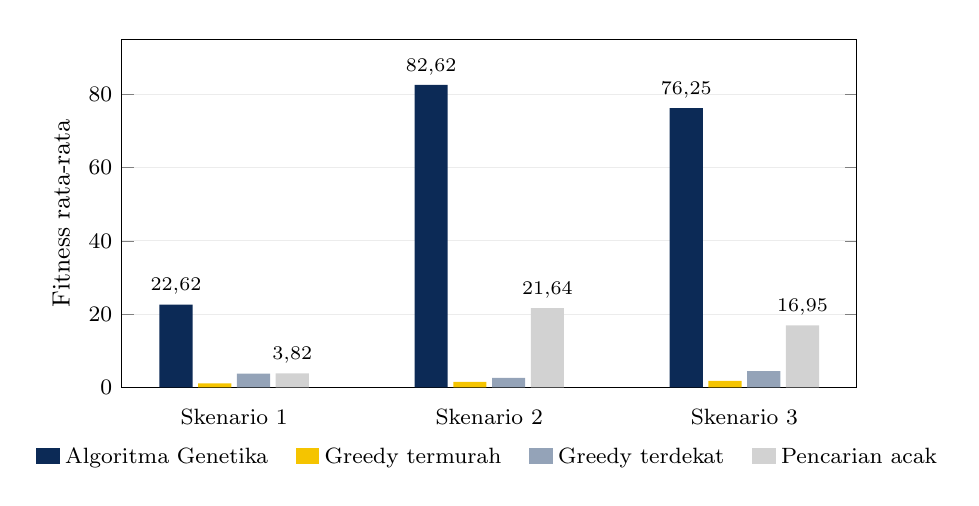
\begin{tikzpicture}
\begin{axis}[
  ybar, bar width=12pt, width=0.9\linewidth, height=6cm, ymin=0, ymax=95,
  symbolic x coords={Skenario 1, Skenario 2, Skenario 3}, xtick=data, xtick style={draw=none}, enlarge x limits=0.22,
  ylabel={Fitness rata-rata}, nodes near coords style={font=\scriptsize, /pgf/number format/use comma},
  legend style={at={(0.5,-0.14)}, anchor=north, legend columns=4, font=\footnotesize, draw=none, /tikz/every even column/.append style={column sep=8pt}},
  legend image code/.code={\draw[#1, draw=none] (0cm,-0.08cm) rectangle (0.3cm,0.12cm);},
  tick label style={font=\footnotesize}, label style={font=\small}, ymajorgrids, grid style={gray!15}]
\addplot[fill=ugmnavy, draw=none, nodes near coords] coordinates {(Skenario 1,22.62) (Skenario 2,82.62) (Skenario 3,76.25)};
\addplot[fill=ugmgold, draw=none] coordinates {(Skenario 1,1.09) (Skenario 2,1.50) (Skenario 3,1.80)};
\addplot[fill=abu, draw=none] coordinates {(Skenario 1,3.77) (Skenario 2,2.62) (Skenario 3,4.41)};
\addplot[fill=gray!35, draw=none, nodes near coords] coordinates {(Skenario 1,3.82) (Skenario 2,21.64) (Skenario 3,16.95)};
\legend{Algoritma Genetika, Greedy termurah, Greedy terdekat, Pencarian acak}
\end{axis}
\end{tikzpicture}
\caption{Fitness rata-rata setiap metode (20 seed per skenario).}
\label{fig:banding}
\end{figure}

\subsection{Sensitivitas Parameter}

\Tabelref{tab:sensitivitas} dan \Gambarref{fig:sensitivitas} memperlihatkan pengaruh tiap parameter pada skenario 1 (10 seed per nilai). Semua run menghasilkan rencana valid.

\begin{table}[H]
\centering
\caption{Fitness rata-rata $\pm$ simpangan baku dan waktu per run. Tebal = nilai bawaan.}
\label{tab:sensitivitas}
\small
\begin{tabular}{@{}l c c c c@{}}
\toprule
\textbf{Ukuran populasi} & 25 & 50 & \textbf{100} & 200 \\
\midrule
Fitness & 18,04 $\pm$ 9,12 & 20,08 $\pm$ 6,94 & \textbf{21,54} $\pm$ 5,26 & 24,53 $\pm$ 4,32 \\
Waktu & 179 ms & 412 ms & 609 ms & 1.376 ms \\
\midrule
\textbf{Peluang mutasi} & 0,01 & \textbf{0,05} & 0,1 & 0,2 \\
\midrule
Fitness & 20,77 $\pm$ 12,66 & \textbf{21,54} $\pm$ 5,26 & 22,58 $\pm$ 9,66 & 14,86 $\pm$ 4,17 \\
Waktu & 409 ms & 609 ms & 759 ms & 883 ms \\
\midrule
\textbf{Peluang crossover} & 0,4 & 0,6 & \textbf{0,8} & 0,95 \\
\midrule
Fitness & 24,23 $\pm$ 6,56 & 26,55 $\pm$ 8,90 & \textbf{21,54} $\pm$ 5,26 & 23,57 $\pm$ 5,71 \\
Waktu & 446 ms & 406 ms & 480 ms & 458 ms \\
\bottomrule
\end{tabular}
\end{table}

\begin{figure}[H]
\centering
\pgfplotsset{sens/.style={width=5.4cm, height=4.2cm, ymin=0, ymax=40, symbolic x coords={a,b,c,d}, xtick=data,
  tick label style={font=\scriptsize}, label style={font=\footnotesize}, title style={font=\footnotesize\bfseries}, ymajorgrids, grid style={gray!15}}}
\begin{tikzpicture}
\begin{axis}[sens, title={Ukuran populasi}, ylabel={Fitness}, xticklabels={25, 50, 100, 200}]
\addplot[ugmnavy, thick, mark=*, error bars/.cd, y dir=both, y explicit] coordinates {(a,18.04) +- (0,9.12) (b,20.08) +- (0,6.94) (c,21.54) +- (0,5.26) (d,24.53) +- (0,4.32)};
\end{axis}
\end{tikzpicture}\hfill
\begin{tikzpicture}
\begin{axis}[sens, title={Peluang mutasi}, xticklabels={0{,}01, 0{,}05, 0{,}1, 0{,}2}]
\addplot[ugmnavy, thick, mark=*, error bars/.cd, y dir=both, y explicit] coordinates {(a,20.77) +- (0,12.66) (b,21.54) +- (0,5.26) (c,22.58) +- (0,9.66) (d,14.86) +- (0,4.17)};
\end{axis}
\end{tikzpicture}\hfill
\begin{tikzpicture}
\begin{axis}[sens, title={Peluang crossover}, xticklabels={0{,}4, 0{,}6, 0{,}8, 0{,}95}]
\addplot[ugmnavy, thick, mark=*, error bars/.cd, y dir=both, y explicit] coordinates {(a,24.23) +- (0,6.56) (b,26.55) +- (0,8.90) (c,21.54) +- (0,5.26) (d,23.57) +- (0,5.71)};
\end{axis}
\end{tikzpicture}
\caption{Fitness rata-rata $\pm$ simpangan baku terhadap nilai parameter (skenario 1, 10 seed).}
\label{fig:sensitivitas}
\end{figure}

\section{Pembahasan}
\label{sec:pembahasan}

\subsection{Mengapa GA Unggul}

Kedua varian greedy terjebak pada satu kriteria lokal. \textbf{Greedy termurah} memilih destinasi gratis dan murah lebih dulu, sehingga waktunya sudah habis (30,6 jam) ketika biayanya baru Rp216.345 dari anggaran Rp1.000.000. \textit{Cost score}-nya sekitar 0,78, jadi fitness-nya rendah. \textbf{Greedy terdekat} bergantung pada titik awal dan tidak pernah menukar pilihan yang sudah diambil, sehingga rata-rata hanya mengisi 28,7 jam dan Rp847.777. \textbf{Pencarian acak} melompat ke destinasi yang berjauhan sehingga biaya taksi membengkak. Dengan jumlah evaluasi yang sama, fitness terbaiknya hanya 3,82 pada skenario 1. Artinya, keunggulan GA tidak berasal dari banyaknya evaluasi, tetapi dari pencarian yang terarah oleh seleksi, crossover, dan mutasi.

Pada skenario 1, GA rata-rata memakai Rp996.297 (99,6\% anggaran) dan 33,9 jam (96,9\% batas waktu) tanpa melanggar keduanya. Ini adalah titik ``paling seimbang'' yang dicari fungsi fitness. Fitness skenario 1 lebih rendah daripada skenario 2 dan 3 karena untuk mengisi 35 jam dibutuhkan sekitar 22 destinasi, sehingga kombinasi yang harus disusun jauh lebih banyak.

\subsection{Peran Komponen GA}

Representasi dua bagian membuat setiap kromosom selalu sah, sehingga tidak ada evaluasi yang terbuang untuk rute rusak. Order crossover mempertahankan urutan relatif dari induk, sehingga potongan rute yang efisien dapat diwariskan. Greedy seeding memberi titik awal yang valid (44\% individu generasi awal valid), tetapi GA tetap memperbaikinya: fitness terbaik naik 4,3 kali dari generasi awal dan perbaikan pertama terjadi pada generasi 13. Elitisme menjamin rencana terbaik tidak hilang, sedangkan mutasi tambah-lokal menambah destinasi di sekitar rute alih-alih di lokasi acak yang jauh.

\subsection{Sensitivitas Parameter}

\begin{itemize}
  \item \textbf{Ukuran populasi.} Populasi lebih besar memberi fitness lebih tinggi dan lebih konsisten (18,04 $\pm$ 9,12 pada 25 individu, 24,53 $\pm$ 4,32 pada 200 individu), tetapi waktunya naik 7,7 kali. Nilai bawaan 100 menjaga waktu tetap di bawah satu detik.
  \item \textbf{Peluang mutasi.} Mutasi 0,2 terlalu merusak dan menurunkan fitness menjadi 14,86. Nilai 0,01--0,1 memberi rata-rata yang mirip, tetapi 0,01 sangat tidak konsisten (simpangan baku 12,66) karena populasi cepat seragam. Nilai bawaan 0,05 memberi hasil paling konsisten.
  \item \textbf{Peluang crossover.} Tidak ada pola yang jelas. Nilai 0,6 memberi rata-rata tertinggi (26,55), tetapi semua selisihnya masih dalam satu simpangan baku, sehingga dengan 10 seed perbedaannya belum dapat dianggap nyata.
\end{itemize}

\subsection{Keterbatasan}

\begin{itemize}
  \item Data tidak memuat titik awal (hotel), sehingga hanya perjalanan antardestinasi yang dihitung. Jam buka juga belum diperhitungkan karena hanya tersedia untuk 100 dari 201 atraksi.
  \item Status VALID mengikuti total biaya dan durasi. Rencana yang VALID masih bisa membutuhkan hari tambahan pada jadwal harian. Kasus ini diberi penalti dan peringkat lebih rendah, dan pada contoh \Tabelref{tab:top5} kelima rencana muat dalam 5 hari.
  \item Delapan atraksi dengan data rute rusak dikeluarkan. Dua pasangan berjarak 0 di matriks memakai nilai pengganti 15 km dari kode asli, yang terlalu besar untuk pasangan yang bersebelahan.
  \item Contoh validitas pada proposal (rute ID001--ID006 dengan 32 jam dan Rp600.000) bersifat ilustratif. Dengan data asli, enam atraksi pertama berdurasi 11,23 jam dengan biaya Rp1.097.025.
\end{itemize}

\section{Kesimpulan}

\begin{enumerate}
  \item Masalah rekomendasi rencana wisata berhasil dimodelkan sebagai gabungan pemilihan dan pengurutan destinasi. Kromosom dua bagian (\texttt{mask} dan \texttt{order}) selalu menghasilkan rute yang sah, dan fungsi fitness $1/(\text{cost\_score} + \text{duration\_score})$ dengan penalti dan bonus minat mengarahkan GA ke rencana yang valid dan seimbang.
  \item Pada tiga skenario, fitness rata-rata GA 3,8 hingga 5,9 kali lebih tinggi daripada pembanding terbaik (greedy termurah, greedy terdekat, dan pencarian acak dengan jumlah evaluasi yang sama). Semua rekomendasi valid dan dihasilkan dalam waktu kurang dari satu detik.
  \item Populasi yang lebih besar meningkatkan kualitas dengan biaya waktu, peluang mutasi yang terlalu tinggi (0,2) merusak hasil, sedangkan peluang crossover tidak berpengaruh nyata pada rentang 0,4--0,95.
  \item Sistem tersedia sebagai aplikasi web dengan peta rute, jadwal harian, grafik evolusi, halaman eksperimen, dan fitur unggah dataset sendiri, sehingga tidak terbatas pada Jakarta.
\end{enumerate}

Pengembangan selanjutnya dapat menambahkan titik awal penginapan dan jam buka, memakai pendekatan multi-objektif seperti NSGA-II untuk menampilkan pilihan kompromi biaya--durasi secara lengkap, serta menambah jumlah seed agar perbedaan antarparameter dapat diuji secara statistik.


%=======================================================================
% DAFTAR PUSTAKA
%=======================================================================
\begin{thebibliography}{9}
\setlength{\itemsep}{2pt}

\bibitem{bps2024}
Badan Pusat Statistik. (2024). Kunjungan wisatawan mancanegara (wisman) pada Agustus 2024 mencapai 1,34 juta kunjungan, naik 18,30 persen (y-on-y). \url{https://www.bps.go.id/en/pressrelease/2024/10/01/2355/}

\bibitem{davis1985}
Davis, L. (1985). Applying Adaptive Algorithms to Epistatic Domains. \textit{Proceedings of the 9th International Joint Conference on Artificial Intelligence (IJCAI)}, 162--164.

\bibitem{goldberg1989}
Goldberg, D. E. (1989). \textit{Genetic Algorithms in Search, Optimization, and Machine Learning}. Addison-Wesley.

\bibitem{econ2020}
Google, Temasek, dan Bain \& Company. (2020). \textit{e-Conomy SEA 2020: Resilient and racing ahead}. \url{https://www.bain.com/insights/e-conomy-sea-2020}

\bibitem{econ2024}
Google, Temasek, dan Bain \& Company. (2024). \textit{e-Conomy SEA 2024: Profits on the rise, harnessing SEA's advantage}. \url{https://services.google.com/fh/files/misc/e_conomy_sea_2024_report.pdf}

\bibitem{holland1975}
Holland, J. H. (1975). \textit{Adaptation in Natural and Artificial Systems}. University of Michigan Press.

\bibitem{qomariyah2021}
Qomariyah, N. N. dan Kazakov, D. (2021). A genetic-based pairwise trip planner recommender system. \textit{Journal of Big Data}, 8, 77. \url{https://doi.org/10.1186/s40537-021-00470-6}

\bibitem{repo}
Halim, N. M., Qomariyah, N. N., dan Kazakov, D. \textit{GA-pairwise-recommender-system} (data \texttt{jsonAttraction.txt}, \texttt{distanceMatrix.csv}, \texttt{durationMatrix.csv}). \url{https://github.com/nnqomariyah/GA-pairwise-recommender-system}

\end{thebibliography}

\end{document}
